\chapter{Habitat of ice reservoirs}

AIRs cannot be built anywhere. They require an appropriate water source and weather conditions cold enough to
amass a seasonal stock of ice. This imposes several meteorological and topographical requirements for the chosen
construction location. The meteorological requirements can be used to identify favourable regions worldwide
whereas the topographical requirements can be used to pinpoint the construction site within the respective
region. Below we detail these requirements and propose methodologies for finding construction sites satisfying
them. 

\begin{figure}[t]
\centering
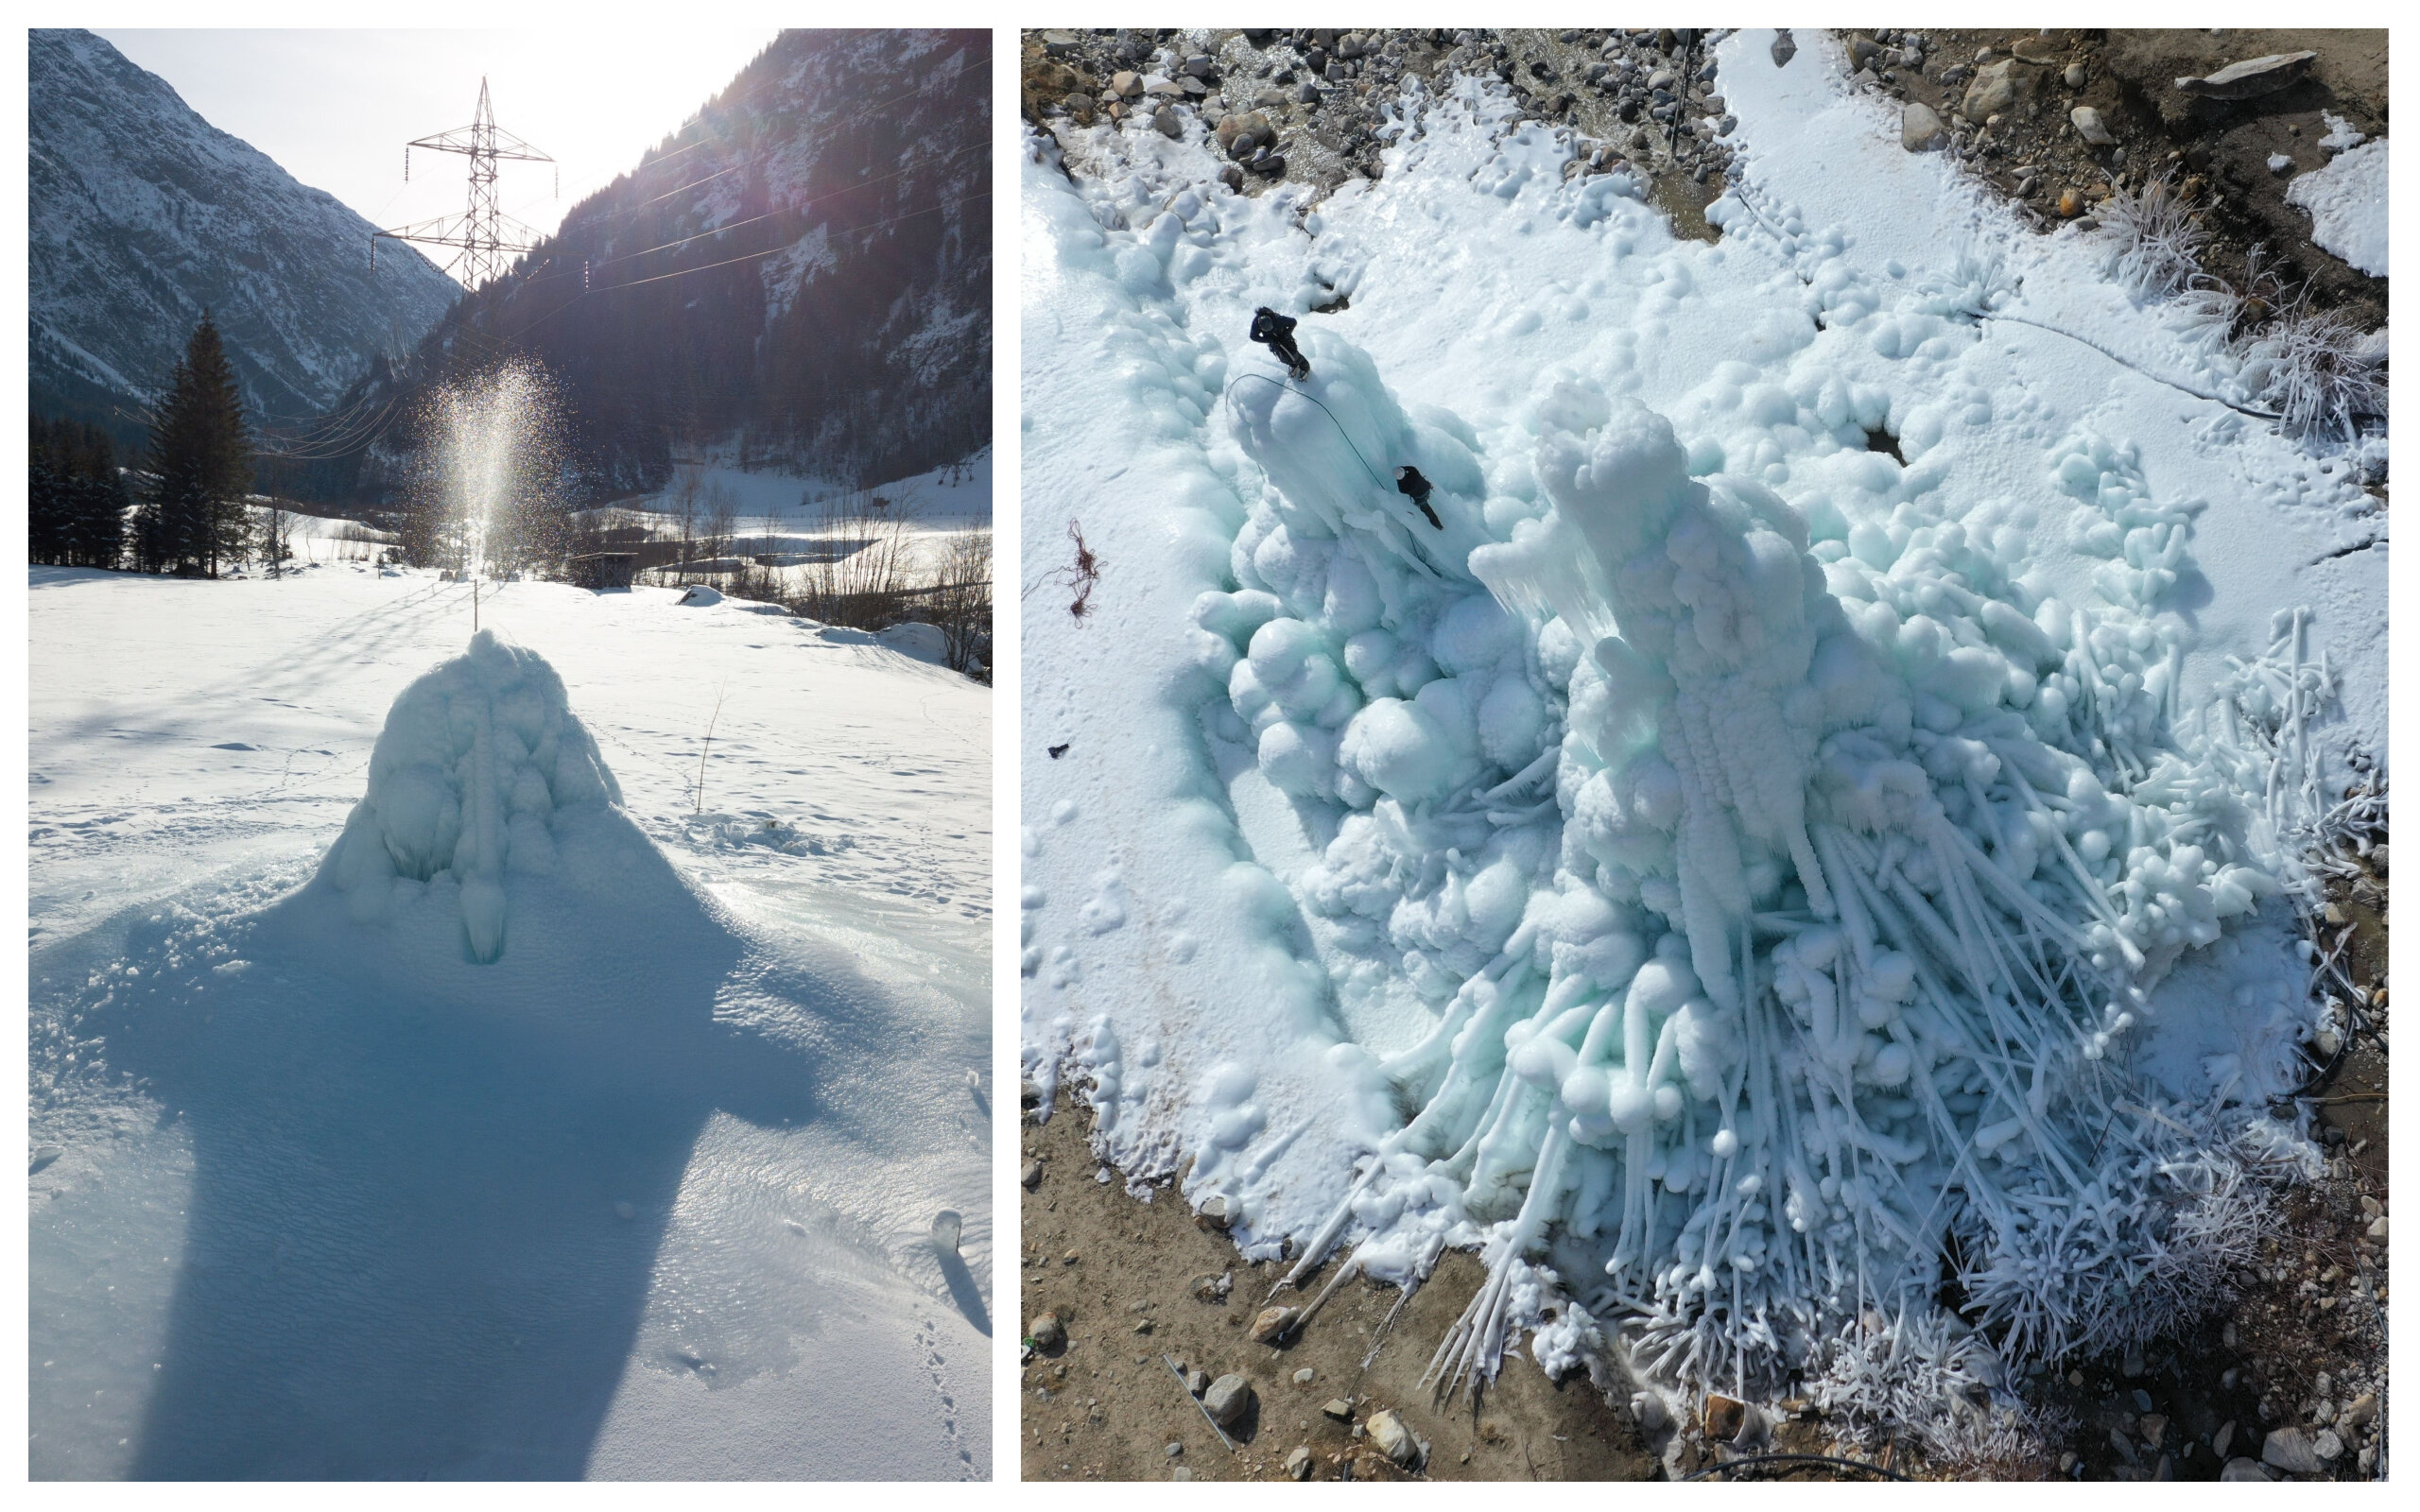
\includegraphics[width=12cm]{Figures/2AIRs.jpg}

\caption{AIRs show significant variation in volume evolution depending on the choice of construction location.}

\label{fig:2AIRs}
\end{figure}

\section{Requirements for AIR construction}

\begin{itemize}
  \item {\bf Water supply} : The water source of an AIR could be either a spring or a stream. Springs are the ideal
    water source since they are easy to transport via pipelines to the construction site due to their relatively
    warm temperatures. Other water sources tend to freeze within the pipeline during tranport. 

  \item {\bf Weather conditions} : AIRs prefer colder, drier and less-cloudy regions.

  \item {\bf Topography} : AIRs prefer shadowed valleys.

\end{itemize}

Different forms of AIRs show different sensitivities to each of these requirements. This is discussed in the
next chapter.

\section{ Checklist for choosing future ice stupa construction site }

\begin{enumerate}

  \item Water source within 10 km of the site.
  \item Mean temperature of construction period less than $- 2 \degree C $.
  \item Number of subzero nights during construction period is greater than 30.
  \item Terrain slope between water source and site greater than 10 m every km. 

\end{enumerate}

\section{ Metrics to compare between two sites}

\begin{enumerate}

  \item Temperature is lower.
  \item Cloudy days are lower.
  \item Humidity is lower.
  \item Daylight hours is lower.

\end{enumerate}

Such a village can create ice stupa which can grow to millions of litres and supply around 10,000 litres of meltwater for 2 months (April and May). Please contact me if further details are required.



\subsection{Minimum requirements}

Our results have shown that Swiss AIRs cannot function as water reservoirs due to their small size and short
survival duration. Therefore, construction of AIRs should not be carried out in locations with meteorological
conditions less favourable than the Swiss site.

It is not straightforward to compare the meteorological conditions between two sites. A proper comparison
requires the complete set of meteorological variables described in Section ?. In order to circumvent this, we
introduce a new metric that serves as an indicator of the water storage potential of any new site.

However, one indicator of the AIR water storage potential of any new site is the number of subzero hours
annually weighted by 

Another way to locate favourable regions is through occurence of aufeis fields

Naturally occuring aufeis fields and glaciers serve as a good indicator of where ice reservoirs can be made.
